\documentclass[12pt, a4paper]{article}

\usepackage[utf8]{inputenc}
\usepackage{matlab-prettifier, fullpage, amsmath,graphicx,float, subcaption,listings,enumitem, setspace}
\usepackage[backend = biber, style = apa, natbib = true]{biblatex} % referencing style
\usepackage[font = footnotesize, labelfont = bf]{caption} % might get rid of the load type. This is just to make it smaller to type more into captions
\DeclareLanguageMapping{english}{english-apa}


\newcommand{\blackbar}{{\nointerlineskip
{\rule{\linewidth}{1mm}}\\}}
\renewcommand{\d}{\textrm{d}}
\newcommand{\mn}[1]{\texttt{#1}}
\renewcommand{\thesection}{\Roman{section}} 
\newcommand{\PK}{PKM$\zeta$ }
\newcommand{\pk}{\PK}
\newcommand{\mPK}{\textrm{PKM}\zeta}
\newcommand{\insertMatlab}[1]{\lstinputlisting[style = Matlab-editor]{#1}}
\newcommand{\citeapa}[1]{(\citeauthor{#1}, \citeyear{#1})}
\newcommand{\derv}[1]{\frac{d#1}{dt}}

\font\myfont=cmr12 at 30pt

\addbibresource{references.bib}

\begin{document}

\begin{titlepage}
\centering
\vspace*{5cm}
{\myfont Who even knows}\\
\vspace{1cm}
\Large{AMATH 423}\\
\vspace{1cm}
\Huge{Oliver Speltz, Levi Davis}\normalsize\\
\vspace{1cm}
\large{March 2019}\normalsize

\end{titlepage}
\doublespacing
\section*{Abstract}
\blackbar

\section*{Background}
\blackbar
The formation of memories and learning in neuroscience has long been a topic of interest. The massive web of neurons in the brain is able to make new memories and learn from information very quickly. We know that neurons exchange information through action potentials transferred through their axons. Recent research has revealed a key aspect of neuronal memory is the maintenance of axonal connections, called synapses (\large{\textbf{Need a citation?}})\normalsize. The dendrites of neurons are connected to the axons of others and they are able to send signals to each other by way of the synaptic cleft that joins them. 

Dendrites of neurons are not static; neurons are part of a highly dynamic system, readily changing connectivity and strength between connected components, owing to a large field focused on the plasiticty of neurons. Connections to new neurons can be formed by the process of \emph{dendritic remodeling}. A core part of dendrites are the dendritic spines, where most excitatory stimuli are applied to, suggesting that spines are a principal component of neuronal circuits \citeapa{dendriticspines}. Although their role remains unclear, general theories focus on their biochemical compartmentalization. A small spine head is located at the tip of the spine, where excitory synapse is located, spatially separating the main body of dendrite from spine cytoplasm \citeapa{dendriticspines}$^{10}$. This separation hinders biochemical diffusion to main dendrite, with majority of diffusion occurring through the spine. During electric stimulus, these spines accumulate calcium and compartmentalize them inside their heads, and are thought to be behind input specific neuro-plasticity \citeapa{dendriticspines}. Longer necked spines have been found to decrease excitory synaptic amplitudes are inversely correlated with length of spine, thereby reducing the voltage contributions to main body of dendrite and, by association, dendritic remodeling. 

To trigger dendritic remodeling, the main school of thought pertains to a counterbalance system of Long Term Potentiation (LTP) and Long Term Depression (LTD). LTP strengthens synpases, increasing transitivity of stimuli between connected neurons. It is considered to be the underlying mechanism for building memories and learning. Whereas LTD is the complement of LTP, wherein a reduction in synaptic strength occurs, lasting hours or longer \citeapa{LTDPaper}. These conjugate pairs work together to optimize the efficiency of synaptic structures. Fundamentally, if LTD was not present, then LTP increase in strength would continue to increase all synaptic bonds until the efficiency between any two pairs is inconsequential. Thus a need for LTD to regulate the other connections is significant. Persistent forms of LTP and LTD require plasticity related proteins, accumulating at synapses for either induction or maintenance. Some molecules have been identified in LTP and LTD maintenance, such as calcium/calmodulin dependent kinase II (CaMKII) for LTP \citeapa{actinDynamics}. 

After persistent LTP or LTD, the process of dendritic remodeling occurs, imploring a combination of functional and structural modifications. The monomer actin is a crucial component of these modifications, and is known to be a core element in spine's cytoskeleton \citeapa{actin_spine}. Polymerization of actin has been shown to be critical in induction and regulation of synaptic plasticity. Recent research suggests inhibition of actin de-polymerization blocks induction of LTD, thereby implying resistance to LTD action during actin polymerization \citeapa{actinDynamics}. Likewise the inhibition of polymerization allows LTD expression and maintenance. G-actin is a component of the cytoskeleton, found in many types of moving cells, F-actin is its polymerized form. F-actin can be used to reshape and move cells, such as forming new synaptic bonds. Furthermore, recent evidence suggests increase in F-actin is needed for LTP induction and decrease in LTD \citeapa{actinDynamics}. Notably, CaMKII has also been identified to play a role in actin regulation, supporting notion of actin playing a role in synaptic plasticity. 

Studies on the Protein Kinase M$\zeta$ (\PK), a brain specific protein kinase C isoform, have revealed it plays a key role in the maintenance of new synapses \citeapa{pkmZeta}. It has been shown to lead to LTP by augmenting excitory postsynaptic currents (EPSCs) via stabilization of AMPA glutamate receptors. mRNA expression of \PK is found in many brain regions, and tends to localize at dendritic spines \citeapa{pkmZeta}. The fast translation of \PK, within 10 minutes of LTP inducing stimuli, constituting a positive feedback type of loop. 

A group hypothesized this system having a bistable bifurcation, leading to a basis for cellular memory (all or nothing approach). This approach fits with hippocampal LTP, wherein a LTP inducing stimuli trigger a calcium increase in spines. After which, CaMKII and other kinases induce long lasting \PK expression in a bistable manner \citeapa{pkmZeta}. Here, their same model for \PK expression is reviewed and explored. 



\section*{Models}
\blackbar
The model proposed by Ogasawara et al is given by equations \ref{pkmeqn}, \ref{acteqn} and \ref{rnaeqn}. It is a system of 3 ordinary differential equations that they proposed due to existing evidence and research. The schematic in Figure \ref{pathway} describes the system as they assumed it. 
\begin{figure}[H]
    \centering
    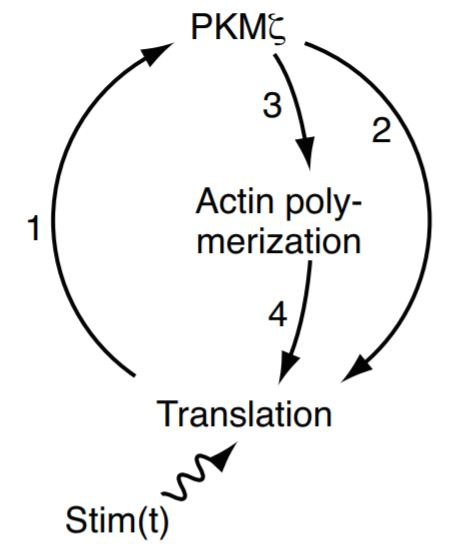
\includegraphics{pics/pathway.JPG}
    \caption{A schematic for the dynamics of the system. \PK stimulates its own translation (arrow 2), as well as F actin polymerization (arrow 3). F actin facilitates protein synthesis in general (arrow 4).}
    \label{pathway}
\end{figure}
The actual pathways of this system are currently unknown, so the authors assumed a simple pathway. Here, Stim(t) represents the collective time dependent stimuli of CaMKII, PKC and MAPK. All of these proteins stimulate \PK in different ways, however for simplicity of the model, the authors included it all as one. Arrow 1 represents the translation of \PK mRNA into functional protein. Arrow 2 represents \PK stimulating its own translation. This positive feedback loop behavior has been shown experimentally \citeapa{pkmZeta}. Arrow 3 represents \pk stimulating actin polymerization, this is not known to be true but is presumed by many researchers \citeapa{pkmZeta}. Finally arrow 4 represents the facilitation by F-actin polymers of all translational activty \citeapa{pkmZeta}. Using this pathway, Ogasawara et al created the ODEs \ref{pkmeqn}, \ref{acteqn} and \ref{rnaeqn}.
\begin{align}
\tau_1\frac{\d P}{\d t} &= j_1R(1-P)-P \label{pkmeqn} \\
\tau_2\frac{\d F}{\d t} &= (j_2 + j_3P)(1-F)-F \label{acteqn}\\
\tau_3\frac{\d R}{\d t} &= j_4F(P+S(t))(1-R) \label{rnaeqn} -R
\end{align}
$P$ represents the concentration of \pk in the cell, it is a unitless quantity, as are all of the other variables of the system. The variables were made unitless because the literature is currently lacking enough data for real numbers to be put to them. $P$ concentration is assumed to max out at 1, due to resource limitations. $j_1$ then represents the translation rate of \pk relative to its degradation rate. $R$ represents the concentration of \emph{active} \pk mRNA, that is, the concentration of \pk mRNA that is being actively translated into protein, $j_4$ is rate at which mRNA is taken into translational machinery (relative to its degradation rate). $S(t)$ is the time dependent stimulus that induces translation of \pk mRNA. $F$ represents the concentration of actin monomers that are associated into F-actin. $j_2$ and $j_3$ are then the rates of actin polymerization independent of \pk and dependent on \pk respectively, both are relative to F-actin dissociation. Total concentrations of actin and \pk mRNA have been shown to be constant throughout the onset of LTP \citeapa{pkmZeta}, so these quantities also max out at 1. The $\tau_i$ terms are included so that the dynamics happen on realistic time scales (on the order of minutes and hours).

Using this model, Ogasawara et al found the system to be very bistable. In wide ranges of the parameters $j_i$, $j_2$, $j_3$ and $j_4$ the system had three equilibrium points, two stable ones separated by an unstable point. The $\tau$ parameters had no effect on the equilibria of the system. We solved the system of ODEs to find the equilibrium points of $P$, $P^*$. 
\begin{gather*}
    P_1^* = 0\\
    P^*_2 = \frac{(1 + j_2j_4 + j_3) + \sqrt{(1+j_2j_4 + j_3)^2 + 4j_3j_4(j_1j_4-j_2-1)}}{-2j_3j_4}\\
    P^*_3 =\frac{(1 + j_2j_4 + j_3) - \sqrt{(1+j_2j_4 + j_3)^2 + 4j_3j_4(j_1j_4-j_2-1)}}{-2j_3j_4}
\end{gather*}

Figure \ref{bifur} shows a bifurcation analysis done by Ogasawara et al. The solid lines represent stable equilibria and the dashed lines represent unstable equilibria. The solid line at 0 is stable until the the transcritical bifurcation when $P_3^*$ collides with $P^*_1$. $P_2^*$ is always stable when it exists.
\begin{figure}[H]
    \centering
    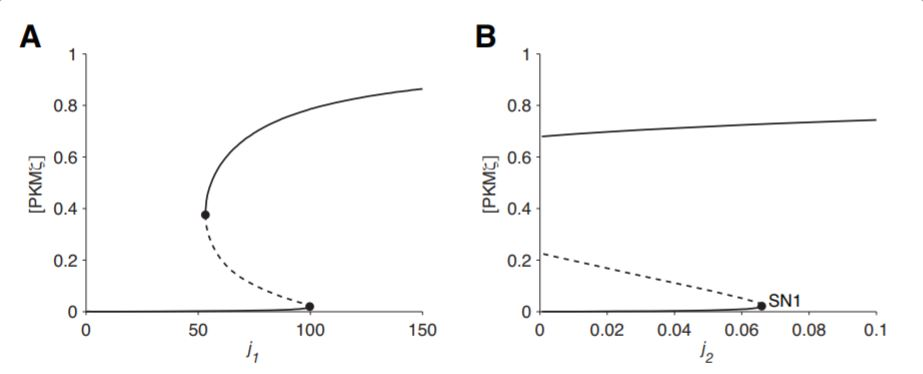
\includegraphics[width = \textwidth]{pics/bifurcations.JPG}
    \caption{Saddle node bifurcations of the system with regards to varying $j_1$ and $j_2$, the translation rate of \pk and the \pk independent polymerization rate of F-actin, respectively.}
    \label{bifur}
\end{figure}

$P^*_1$ then represents the steady state associated with no LTP, $P^*_2$ is the state associated with \pk presence and LTP. We will refer to them as the \emph{on} and \emph{off} states of the system. 

Ogasawara et al then investigated the amount of stimulus to put in to a cell in the off state to have it be put into the on state. They found that if the stimulus was too weak or not for a long enough period of time, the levels of \pk would rise transiently, then return to the off state when the stimulus went away. Stronger or longer stimuli would result in the system asymptotically approaching the on state and even stronger stimuli caused the system to overshoot the on state and approach it asymptotically from above.

Ogasawara et al provided some credibility for their model by using to recreate the findings of various studies involving the \pk pathway. In one study, it was shown that the ZIP inhibitor can reverse LTP \citeapa{ZIPbois}. To simulate this using their model, they started with the system in the on state, then mimiced ZIP inhibition by forcing \pk to be 0 for 60 minutes. They found that it did confirm the results and the levels of \pk did not return to the on state. 

Another test of the model was to see how it responded to actin inhibitors. Actin polymerization inhibitors have been shown to prevent the onset of LTP \citeapa{actin_bois}. In recreating this, Ogasawara set both $j_2$ and $j_3$ to zero, simulating actin failing to polymerize. They found that stimuli that would send a normal cell in the off state into the on state failed to do the same with this inhibited system. This highlights that the extra feedback of actin on the system is essential to the bistability of the system. The feedback of \pk on itself is insufficient alone. 

In extending this model, we were interested to see what it would take to turn a cell in the on state back off. The plasticity of neurons is essential for learning new information, so a cell in LTP must have some way to exit it in a controlled manner. We hypothesized that there is possibly some natural inhibitor of \pk translation that could serve to take a cell out of LTP when it is needed. We incorporated into the model a new stimulus $S_2(t)$ which, when it is present, serves to slow down the rate of \pk translation. The updated model only changes the equation for \pk mRNA, which is given now,
\begin{equation}
    \tau_3\frac{\d R}{\d t} = \frac{j_4F(P+S_1(t))(1-R)}{1 + S_2(t)} -R.
\end{equation}
This was designed based off of other repressor/inhibitor models we have seen before. The equations for \pk itself (\ref{pkmeqn}) and F-actin (\ref{acteqn}) remained the same as the original model. Proceeding forward this model will be referred to as the Off-Toggle Model.

We also hypothesized of a resistance to actin polymerization, correlating to the impedance associated with dendritic spines. For simplicity sake, a new term was added to the system, HS, dependent on actin polymerization and inhibiting mRNA transcription for \PK. Our preliminary theory is inclusion of this new term will attenuate and add a delay for the \PK response. This model will be referred to as the Inhibition Model onward. The ODE representation for this model is 
\begin{align*}
    \derv{P} =& j_1R(1-P)-P\\
    \derv{F} =& (j_2+j_3P)(1-F)-F\\
    \derv{R} =& \frac{j_4F(P + Stim(t))(1-R)}{1+j_5HS} - R\\
    \derv{HS} =& j_6F(1-HS) - HS
\end{align*}
Notably the only difference in this model relative to the base model by Ogasawara et al is the last ODE and the denominator for mRNA's ODE. This too was designed based off inhibitor models seen in the past, with a strength weighting of $j_5$ since HS is bounded by 1 (arbitrary units). 
% \begin{align*}
% \frac{\d P}{\d t} &= j_1R(1-P)-P \\
% \frac{\d F}{\d t} &= (j_2 + j_3P)(1-F)-F \\
% \frac{\d R}{\d t} &= \frac{j_4F(P+S_1(t))(1-R)}{1 + S_2(t)} -R
% \end{align*}

% \begin{align*}
% \frac{\d P}{\d t} &= j_1R(1-P)-P \\
% \frac{\d F}{\d t} &= (j_2 + j_3P)(1-F)-F \\
% \frac{\d R}{\d t} &= \frac{j_4F(P+S(t))(1-R)}{1+j_5HS} -R \\
% \frac{\d HS}{\d t} &= j_6F(1-F) - HS 
% \end{align*}


\section*{Results}
\blackbar

To ensure that our models did not alter the dynamics of the original model they were based off of, we tested our models by weighting the new term by 0, effectively turning off the inhibition term or stimulation. Results can be seen in figure \ref{fig:aresame}.
\begin{figure}[H]
    \centering
    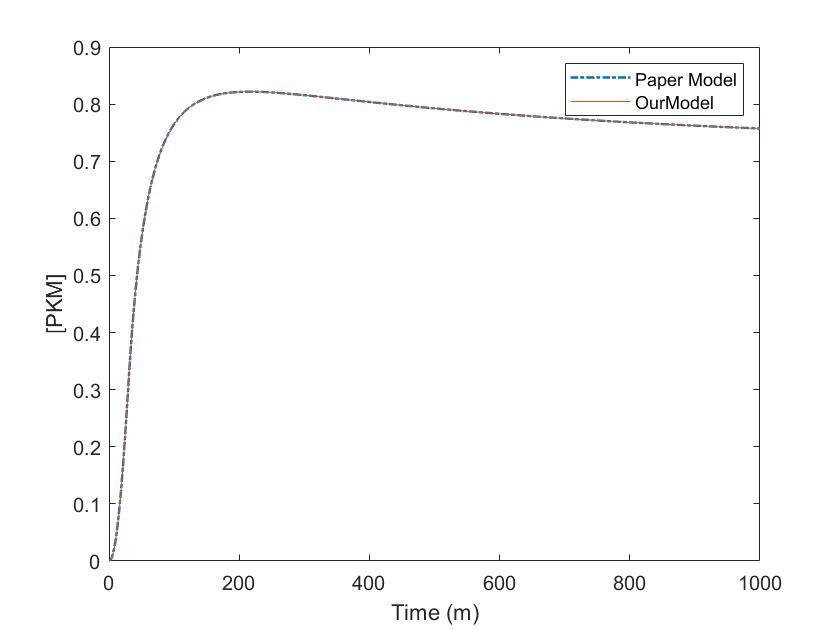
\includegraphics[scale = 0.4]{pics/toggleSwitch_Agrees_withPaper.jpg}
    \caption{Reassurance that new model additions did not change behavior of solution depicted in base model. All attempted models had same behavior when using default parameters. Only one test is depicted however.}
    \label{fig:aresame}
\end{figure}
However, for the actin resistance models, the steady states did change. Small inclusions of the new species $HS$ reduced the amplitude of \PK steady states, and did not drastically alter the bifurcation. Any incorporation of inhibition resulted in shifting the bifurcation curve, seen in figures \ref{fig::smallj5}-\ref{fig:largej5}. The decrease in amplitude agrees with the expected results, that inclusion of a resistance term decreases the strength of \PK signal. What is interesting is that as $j_5$ is increased, the bifurcation shifts to the right and it eventually loses its bistability, seen in figure \ref{fig:largej5}, where the bifurcation becomes unstable and the stability jumps straight to a higher concentration. 

\begin{figure}[H]
    \centering
    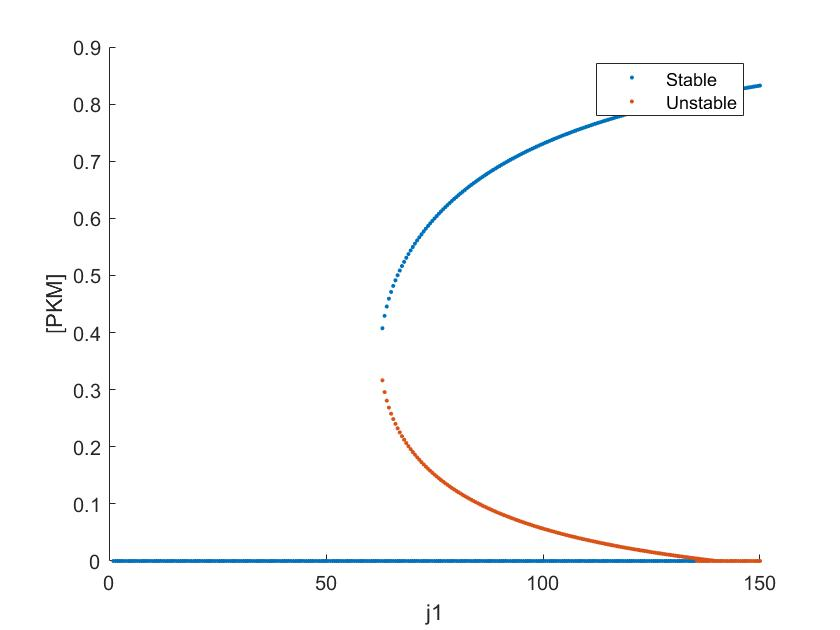
\includegraphics[width = 0.5\textwidth]{pics/inhibition_smallj5.jpg}
    \hspace*{-0.9em}
    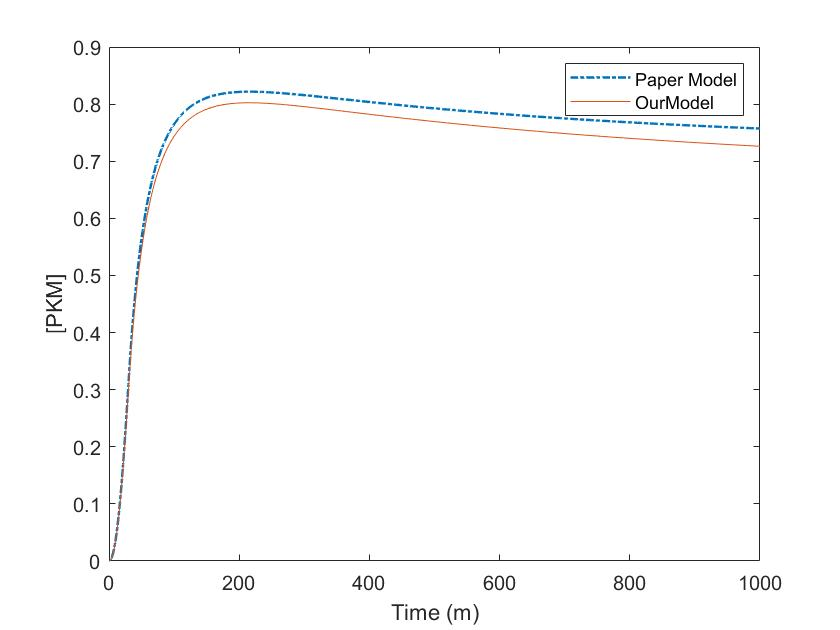
\includegraphics[width = 0.5\textwidth]{pics/inhibition_smallj5ODE.jpg}
    \caption{Steady state bifurcation diagram while keeping $j_5 = 0.8$ throughout. The figure on the right is solution to ODEs with $j_1$ at default value, 80.}
    \label{fig::smallj5}
\end{figure}
\begin{figure}[H]
    \centering
    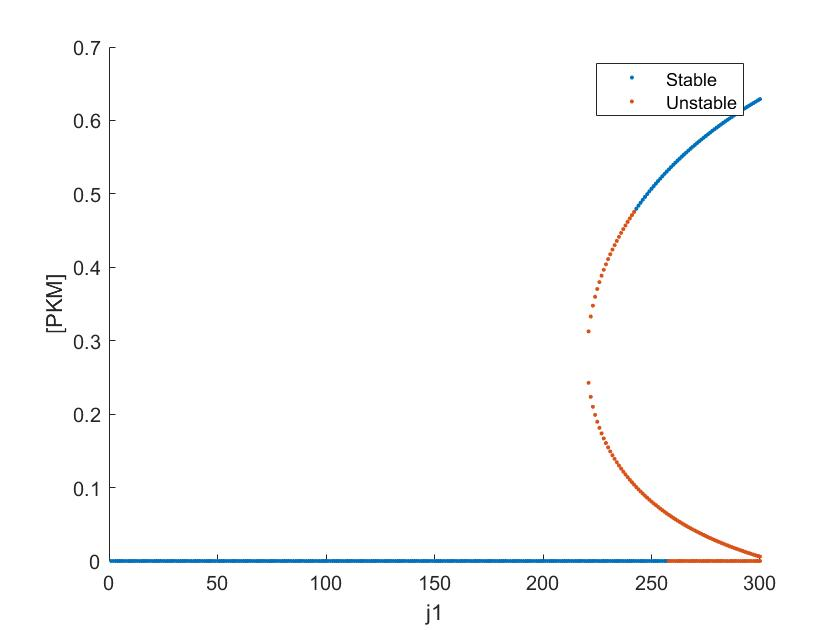
\includegraphics[width = 0.5\textwidth]{pics/inhibition_largej5.jpg}
    \hspace*{-0.9em}
    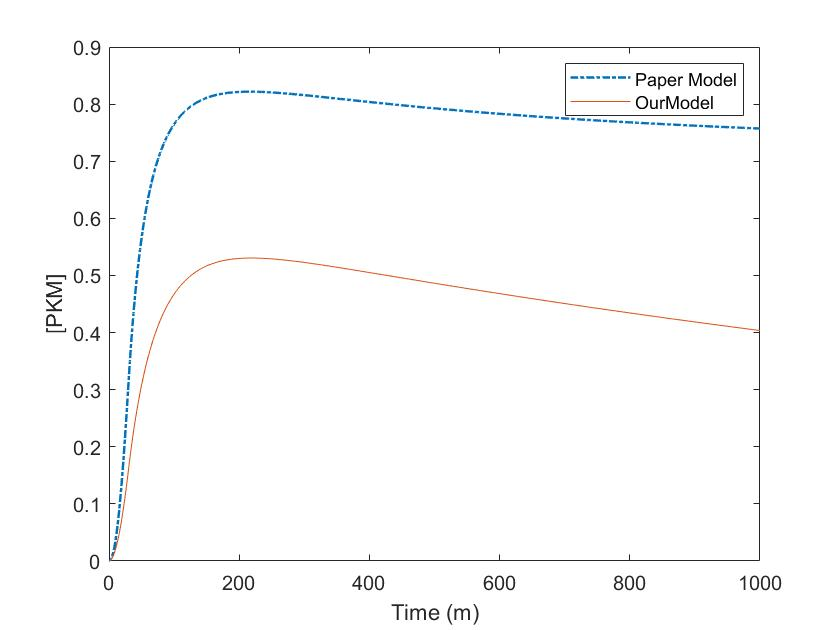
\includegraphics[width = 0.5\textwidth]{pics/inhibition_largej5ODE.jpg}
    \caption{Steady state bifurcation diagram while keeping $j_5$ constant at 5. The figure on the right is solution to ODEs with $j_1$ at default value, 80.}
    \label{fig:largej5}
\end{figure}
Furthermore, ranging $j_5$ also produces a bifurcation, as seen in figure \ref{fig::j5Range}. This suggests that smaller inhibition strength keeps bistability in the system, while reducing amplitude of \PK response.  
\begin{figure}[H]
    \centering
    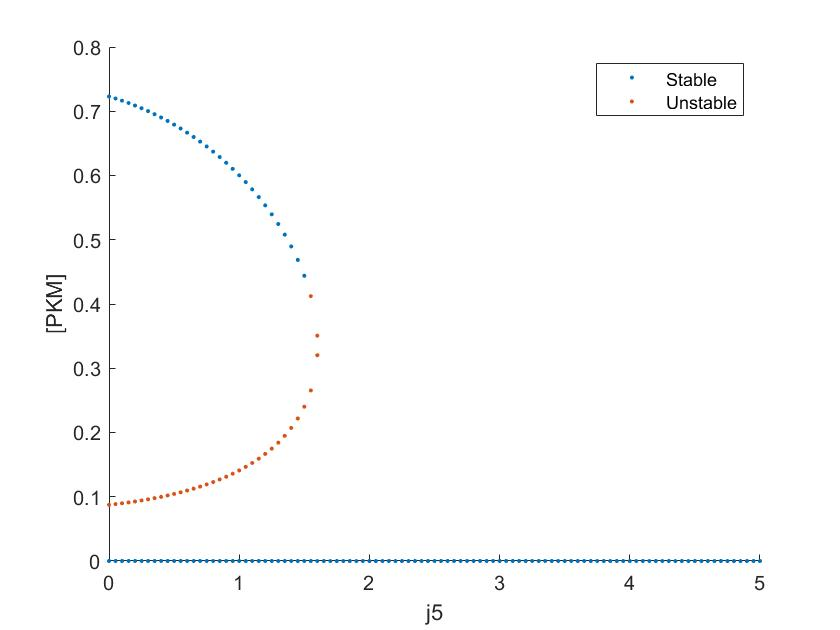
\includegraphics[width = 0.75\textwidth]{pics/inhibition_j5Range.jpg}
    \caption{Bifurcation diagram, ranging $j_5$}
    \label{fig::j5Range}
\end{figure}

In the toggle switch model, exploration of turning off \PK response was explored. To do so, a few feasible approaches were employed, beginning with testing a small stimulant strength for a "short" time period, seen in figure \ref{fig::toggle_shorttime_shortInt}. The time duration was significantly longer than the onset stimulus time, by an order of twice the magnitude. It did not result in toggling off \PK response, rather once the secondary stimulus was applied, it returned to the on toggle state. Exploration for the same time frame but with a higher intensity resulted in a high similarity to a low intensity version. The resultant solution only slightly decreased the amplitude of \PK at the end of the stimulus, figure \ref{fig::toggle_shorttime_highInt}. To ascertain if no stimulus would result in off-toggling the system, a much longer stimulus was applied, figure \ref{fig::toggle_longtime_lowInt}. This indeed toggled off the high response, but resulted in a slow increase, indicating not a complete off-toggle. A study suggesting a low frequency stimulus induces LTD was incorporated, figure \ref{fig::toggle_shortSin}, displaying an oscillatory decay at a slower rate. 

\begin{figure}[H]
    \centering
    \begin{subfigure}[l]{0.5\textwidth}
        \centering
        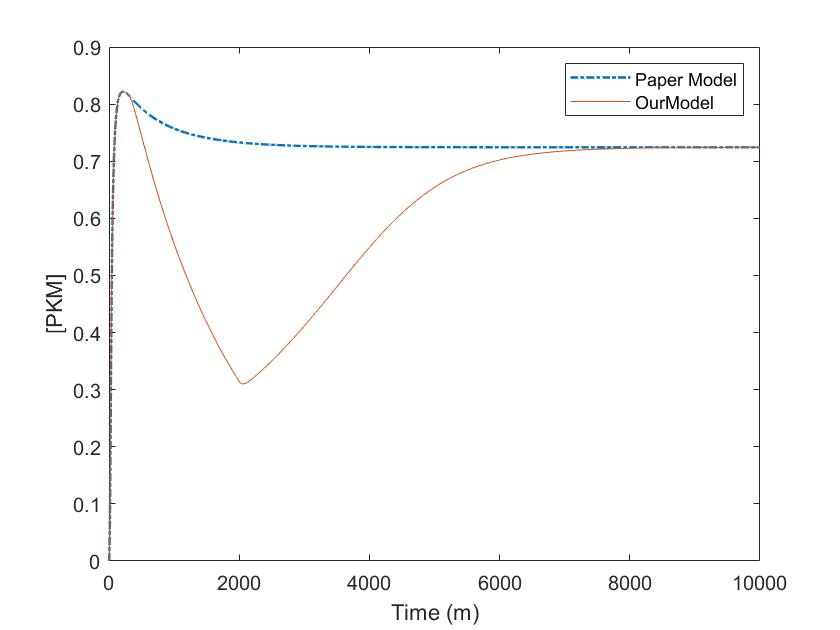
\includegraphics[width=\textwidth]{pics/toggleSwitch_shorterSquareWave.jpg}
        \caption{ }
        \label{fig::toggle_shorttime_shortInt}
    \end{subfigure}
    \hspace*{-0.9em}
    \begin{subfigure}[r]{0.5\textwidth}
        \centering
        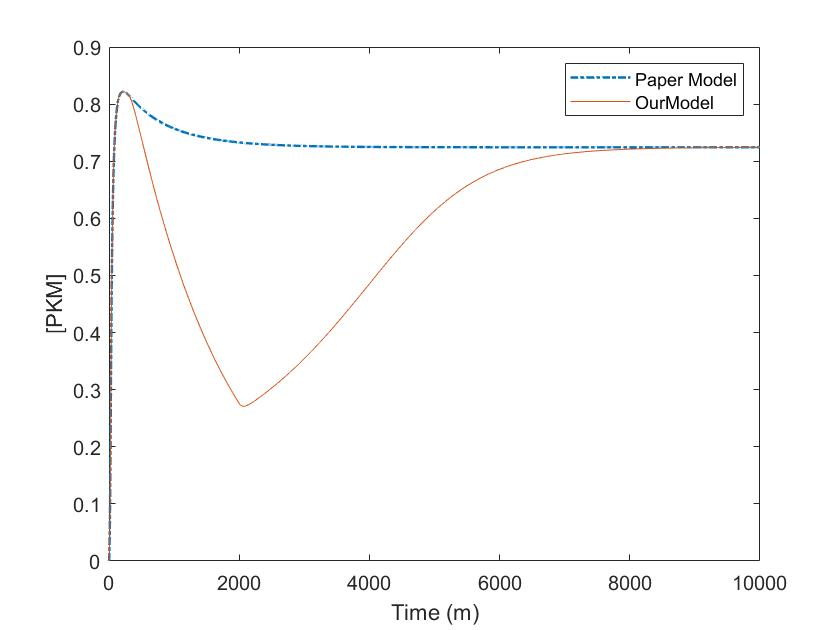
\includegraphics[width =\textwidth] {pics/toggleSwitch_shorterSquareWave_highIntesnity.jpg}
        \caption{ }
        \label{fig::toggle_shorttime_highInt}
    \end{subfigure}
    
    \begin{subfigure}[l]{0.5\textwidth}
        \centering
        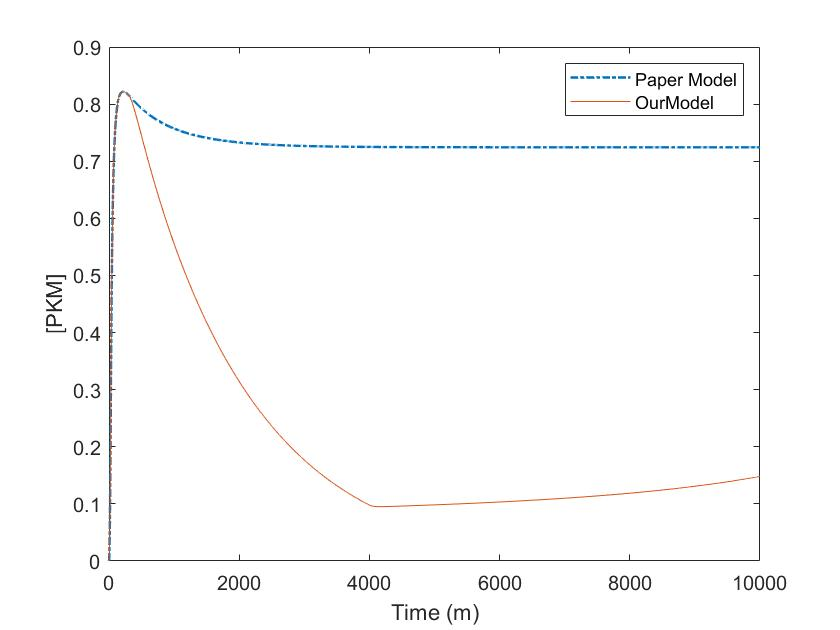
\includegraphics[width = \textwidth]{pics/toggleSwitch_LongSquareWave.jpg}
        \caption{ }
        \label{fig::toggle_longtime_lowInt}
    \end{subfigure}
    \hspace*{-0.9em}
    \begin{subfigure}[r]{0.5\textwidth}
        \centering
        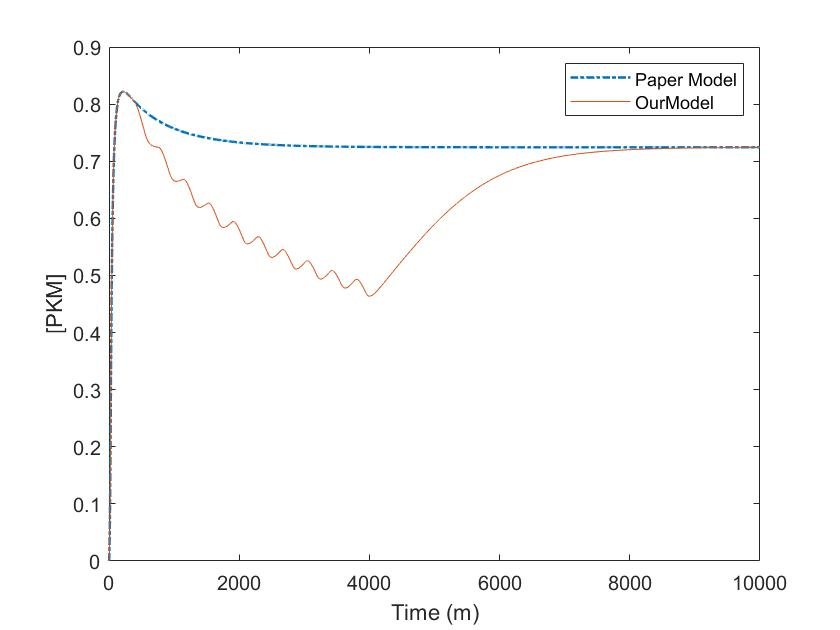
\includegraphics[width = \textwidth]{pics/toggleSwitch_sinpulse_ling.jpg}
        \caption{ }
        \label{fig::toggle_shortSin}
    \end{subfigure}
    \caption{(\ref{fig::toggle_shorttime_shortInt}) "Short" duration, low intensity, secondary stimulus applied to a strong response \PK. The time duration was set at 2000 minutes, with a square wave of intensity 25. (\ref{fig::toggle_shorttime_highInt}) "Short" duration, high intensity response to a secondary stimulus. Time duration for 2000 minutes, square wave of intensity 125. (\ref{fig::toggle_longtime_lowInt}) "Long" duration, low intensity response to a secondary stimulus. Time duration for 4000 minutes, square wave of intensity 25. (\ref{fig::toggle_shortSin}) "Short" duration, low intensity response to a secondary stimulus. Time duration for 2000 minutes, positive portions of a sine wave of intensity 25.}
\end{figure}

\section*{Discussion}
\blackbar

Interestingly, the inhibition model behaved differently than what was anticipated. True, the attenuation was expected, although a delay was not entirely apparent in any parameter mixture. We attribute this to the rapid onset of the ON position from bifurcation. Furthermore, shifting in the bifurcation was an interesting phenomenon, more so when bistability is lost due to the shifting. It becomes clear that if an inhibition term is added to the system, the weight of mRNA replication would have to increase to keep the same dynamics, contributing to the shifting event. Loss of bistability is interesting however. This result suggestest that with increased resistance to \PK, the system loses its all or nothing type of switching, and will trend towards a specific steady state. Due to the simplicity of the model, we expect that this behavior can be extrapolated to refer to decrease in LTP caused by actin inhibitors. Further exploration is needed along with a more realistic model highlighting the significance actin has on LTP and LTD regulation to fully explore the dynamics. 

The off toggle model came at a partial surprise, it was not expected for \PK to have such a strong basin of attraction. Largely we contribute this to the hysteresis shown in figure \ref{bifur}, implying that under normal conditions \PK will not spontaneously revert back to 0 steady state. The use of the secondary stimulus is a forcing function that ignores this restriction and attempts to coerce it to the 0 state. Our findings support that this system is a toggle switch, with a very stable on state, conducive with the literature suggesting a prolonged expression of \PK is required for LTP induction and maintenance. However it does not give an explanation or suggestion for after LTP occurrence, or the mechanistic happenings of how \PK returns to the off state for to await another LTP. We speculate that for this to occur, a separate system needs to be constructed, defining LTD induction, to work in conjunction with this system. Any future work should explore this idea, since neuronal plasticity readily has to be turned on and off to optimize neural network.  


\section*{Conclusion}
\blackbar



\newpage
\begin{singlespace}
\printbibliography
\newpage
\section*{Matlab Appendix}
\insertMatlab{amath423Final.m}
\insertMatlab{computeSSNew.m}
\insertMatlab{neuronFireODE.m}
\insertMatlab{neuronFireODENewTerm.m}
\end{singlespace}
\end{document}
